% Working paper draft. Compile: latexmk -lualatex main.tex (in paper/). Tables come from
% experiments/tables.py (paper/tables/*.tex), figures from experiments/fig1.py to fig4.py and worked_example.py;
% `uv run python -m verifier_gate.experiments.reproduce` regenerates all of them offline (with the Facts archive,
% see the README). Which result file backs which number: results/README.md.
\documentclass[11pt]{article}
\usepackage[a4paper,margin=2.3cm]{geometry}
\usepackage{fontspec}
\setmainfont{Libertinus Serif}
\setsansfont{Libertinus Sans}
\setmonofont[Scale=0.88]{Libertinus Mono}
\usepackage{microtype}
\usepackage{amsmath}
\usepackage{graphicx}
\usepackage{booktabs}
\usepackage{array}
\usepackage{caption}
\captionsetup{font=small,labelfont=bf}
\usepackage[round,authoryear]{natbib}
\usepackage{xcolor}
\usepackage[colorlinks=true,linkcolor=black,citecolor=black,urlcolor=black]{hyperref}
\usepackage{enumitem}
\setlist{itemsep=2pt,topsep=4pt}
\usepackage{float}

\newcommand{\dsl}[1]{\texttt{#1}}

\title{Propose and Prove: A Symbolic Gate for LLM Explanations\\of Glass-Box Credit Models\\[4pt]
\large Evidence from Synthetic and Plasmode Data}
\author{Anton P. Stahl\thanks{Contact: \texttt{anton\_paul.stahl@mailbox.tu-dresden.de}. Code, data, LLM answers and results:
\url{https://github.com/antonpstahl/feasibility-symb-verific-gate-llm-explanation} (private while this is a draft;
access on request).}}
\date{Working paper, draft of 19 October 2026}

\begin{document}
\maketitle

\begin{abstract}
\noindent
Banks that let a large language model (LLM) write explanations of their credit models need a control for the text,
and US model-risk guidance leaves that step to the bank. We present a propose-and-prove gate. The LLM writes an
explanation together with a plan of claims in a small domain-specific language (DSL). A deterministic verifier judges
every claim against the model's exact additive terms and their bootstrap bands, using a lexicon that gives each
explanation word a truth condition: true, false or undecidable. A round trip reads the finished text back into claims
three times, so that what the reader gets, not only the plan, is checked. Failing claims go back to the writer with
their evidence. We test the gate on credit data with a planted truth, a synthetic tier and a plasmode tier built on
real credit features, with an explainable boosting machine (EBM) and depth-2 XGBoost (36 models per tier). On the
oracle, the lexicon's confident errors are at most 0.9\%; on the fitted models, judged against the planted truth, they
reach 2.4\% on synthetic and 4.6\% on real features, mostly because the models themselves err. The verifier stops
every one of 10,720 scripted errors in claim plans; in finished texts the round trip stops 96\%, and its weak spot is
a feature the model does not have. With Claude Haiku~5.5 as the writer, the share of texts that state something false
about the model falls from 20.5\% to 0.16\% with author-reviewed labels (from 58.5\% to 4.5\% as read by an LLM), and
a spot check on 52 adverse-action notices gives 47\% to 4\%. The pre-study's API calls cost \$8.77 in all. With an
archive of the fitted models' facts, one command reproduces every number offline.
\end{abstract}

\section{Introduction}

Model documentation in banks is full of numbers that someone has to put into words. LLMs can write those words, but
they turn precise numbers into imprecise language. In an earlier study of LLM explanations of a glass-box demand
model, over-attribution of near-flat features was the most common failure: they scored 3.70 against 5.00 for
monotonic features on faithfulness, the fifteen fitted interactions carried 30.7\% of the model's importance, and two
LLM judges from different vendors agreed below the conventional threshold on every measure
\citep{stahl2026seminar}. An LLM judge is therefore not a control a model-risk team can rely on.

The regulatory frame makes this the bank's problem. The new US interagency guidance on model risk management
\citep{sr262026} covers the credit model but leaves generative AI out of its scope, so the LLM that describes the model
is not validated with it. Adverse-action notices add a second requirement: the reasons a lender gives must be the
principal reasons for the decision \citep{regb}, and their wording must follow what was measured
\citep{sudjianto2026evidence}. The question a validator asks is simple: how do we know the LLM writes it completely
and correctly? This paper answers with numbers per claim type rather than an argument.

The mechanism is known: an LLM translates into a formal language and a solver checks \citep{gao2023pal,pan2023logiclm,
nezhad2025symcode}, and the round trip from formal to text to formal has been used for verification certificates and
policies \citep{rodriguez2026cycle,an2025neurosymbolic}. Closest to our setting, structured claims with provenance
have been attached to LLM narratives of a gradient-boosted model, but they deliberately avoid strength words,
interactions and uncertainty \citep{kim2026reasoning}, and schema-level gates leave a gap between checked fields and
correct prose \citep{gupta2026veritygate}. Our contribution is the part that is still open:

\begin{enumerate}
\item a \textbf{lexicon} that gives explanation words (\emph{strong}, \emph{mostly increases}, \emph{hardly matters},
\emph{the effect reverses}) truth conditions on the fitted model and its bootstrap bands, with an explicit third value
for what the data do not settle;
\item a \textbf{gate} that checks both the claim plan and the finished text, repairs with evidence, and is evaluated as
a control: the probability that a released text holds a false claim, before and after the gate;
\item \textbf{evidence on planted truth}, on synthetic data and on real credit features with a planted outcome, for two
model classes, global explanations and a local spot check of adverse-action reasons, all reproducible from the
repository.
\end{enumerate}

\section{Related work}

\paragraph{Symbolic bridges.} Program-aided and solver-aided reasoning \citep{gao2023pal,pan2023logiclm} and
verifiable mathematical code \citep{nezhad2025symcode} move errors from opaque text into checkable programs.
Cycle-consistent explanations of verification certificates \citep{rodriguez2026cycle} and redundant formalization of
policy statements \citep{an2025neurosymbolic} show that a text can be read back into a formal object and compared; the
second checks several readings for agreement, as our round trip does. In finance, numerical claims from filings have
been verified with a solver \citep{hall2026verifin}, but against documents, not against a model.

\paragraph{Claims in explanations of models.} Model checking has served as an oracle to test LLM explanations of
policies \citep{gross2026testing}. For tabular models, the closest work attaches claims with provenance to narratives
of stock-return predictions \citep{kim2026reasoning} or gates narrations by schema \citep{gupta2026veritygate}.
Vague language is a known core challenge for explanations in natural language \citep{reiter2019nlg}, and a logically
sound statement can still mislead \citep{chan2026logical}; we add an emphasis rule and coverage for this reason. Data-to-text
work reads facts back out of generated text \citep{wiseman2017challenges}. A distributional view of LLM risk measures
how outputs vary \citep{garcialorite2026distributional}; the gate certifies each output instead. Deterministic gates
need their own evaluation tested \citep{elina2026maat}, which is why we test ours with mutations and planted truth.

\section{Method}

Figure~\ref{fig:loop} shows the loop. The \textbf{fact provider} reads the fitted model $M$ as an exact sum of step
terms: main effects and pairs of an EBM \citep{lou2013ga2m,nori2019interpretml}, or the trees of a depth-2 XGBoost
(XGB2 below; \citealp{chen2016xgboost}), which is also a sum of terms on one or two features. Both are purified with
the functional ANOVA \citep{lengerich2020purifying} and centered on the training sample, so ``the effect of a feature'' means the
same for both models. Uncertainty comes from 100 bootstrap refits with Poisson weights: percentile bands for shares,
ranks and contrasts, and simultaneous (sup-t) bands for whole curves \citep{montielolea2019simultaneous}, which is
what judging a curve's shape needs. The \textbf{handover} shows the writer these facts in a readable form that is
checked against $M$ before use: the facts only (H1), or the facts and the statements the verifier certifies (H2).

\begin{figure}[t]
\centering
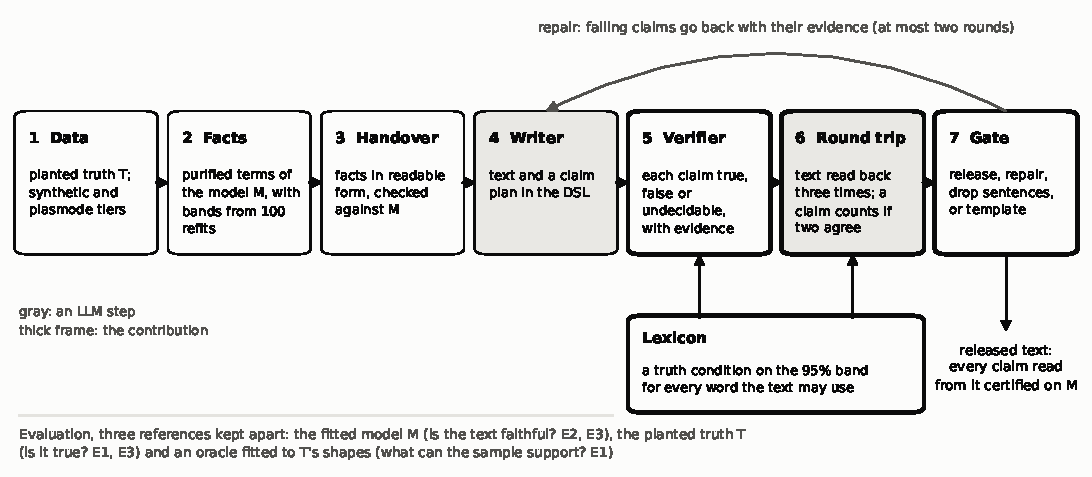
\includegraphics[width=\textwidth]{figures/fig1_loop.pdf}
\caption{The propose-and-prove loop. Gray: an LLM step; thick frame: the contribution. The evaluation keeps three
references apart: the fitted model $M$ (is the text faithful?), the planted truth $T$ (is it true?) and, in E1, an
oracle fitted to the planted shapes (what can the sample support?).}
\label{fig:loop}
\end{figure}

The \textbf{writer} (an LLM) returns sentences and, for each, its claims in the DSL (Table~\ref{tab:dsl}): rank,
share, strength, ``hardly matters'', direction (strict, ``mostly'', or ``generally''), comparisons, a jump or a peak
at a location, and the pattern of an interaction (amplification, sign flip, none). Any claim can be hedged as
\dsl{unsettled(\ldots)}, and neighboring values form sets (``weak to moderate'', ``second or third''). The DSL is
plain Python syntax, parsed with \dsl{ast} against a whitelist, so nothing is executed.

The \textbf{verifier} judges each claim with the \textbf{lexicon}: a claim is true if the whole 95\% band lies inside
the set its word names, false if the band lies outside it, and undecidable otherwise. ``Strong'' means a share of
importance of at least 15\%, with an effect the data can detect; ``mostly increases'' needs a detected reversal on at
most 10\% of the data; ``hardly matters'' needs a share band below 2\%, or no detectable effect, an estimated share
below 2\% and a band below 5\%. Undecidable claims are never released as stated: the writer can hedge them or state
the set the band supports. The lexicon was calibrated on one discovery seed by a rule fixed beforehand; no threshold
moved, and it was frozen before any confirmation run (git tag \dsl{e1-frozen}, commit \dsl{e26c2b9}, with the planted
labels). One change followed, after the writer pilot and before any confirmation run: version~2 judges the location of
a jump or peak on a count feature against the gap between neighboring observed values, so that the step from 0 to 1
delinquency gets the same verdict whether a model cuts at 0.5 or at 1 (\dsl{lexicon-v2}, \dsl{5383c2a}); E1 on the
discovery seed did not change. The writer's and the extractor's prompts were frozen before E3 (\dsl{prompts-v3-x3},
\dsl{cf1ee6b9}).

The \textbf{round trip} reads the finished text back into claims with a second LLM call (the extractor), which sees
neither the plan nor the facts. It reads three times; a claim counts if two readings find it. A claim the text states
beyond its plan is verified like a plan claim; a statement no DSL form expresses blocks the text if it states a
number; every top-3 term and every pair above 10\% of the importance must be covered; and the opening sentence may not
lead with a minor term. The \textbf{gate} releases a text that passes, sends failing claims back with their evidence
and advice (at most two rounds), then drops failing sentences, and as a last resort releases a template built from
certified statements.

\begin{table}[t]
\centering\footnotesize\setlength{\tabcolsep}{4pt}
\caption{The DSL and the lexicon (global claims). The local forms used for adverse-action notices and the full
threshold table are in the appendix (Table~\ref{tab:dsl-local}).}
\label{tab:dsl}
\begin{tabular}{p{3.3cm}p{5.1cm}p{6.4cm}}
\toprule
\textbf{Words in the text} & \textbf{DSL claim} & \textbf{Meaning (judged on the whole 95\% band)} \\
\midrule
“a strong / moderate / weak effect” & \texttt{strength("x") == "strong"} (or “moderate”, “weak”) & share of the model's importance at least 15\% / 5\% to 15\% / 2\% to 5\%, and an effect the data can detect \\
“a weak to moderate effect”, “a moderate to strong effect” & \texttt{strength("x") in ("weak", "moderate")} & the share lies somewhere in the classes named \\
“at most a weak effect”, “a small effect” & \texttt{strength("x") in ("negligible", "weak")} & share below 5\% \\
“hardly matters”, “negligible” & \texttt{negligible("x")} & share below 2\%, or no detectable effect and a small share \\
“the most important”, “the second most important” & \texttt{rank("x") == 1} & rank among the features by importance \\
“second or third”, “among the three most important” & \texttt{rank("x") in (2, 3)}, \texttt{rank("x") in (1, 2, 3)} & one of consecutive ranks \\
“about 30\% of the importance” & \texttt{share("x") == approx(0.30)} & share of importance, within 2 points or 10\% \\
“matters more than” & \texttt{effect("x") > effect("y")} & x's importance exceeds y's \\
“risk increases with x” / “decreases” & \texttt{direction("x") == "increasing"} (or “decreasing”) & rises from the 5th to the 95th percentile, with no reversal the data can detect \\
“risk mostly increases with x” & \texttt{direction("x") == "mostly\_increasing"} (or “mostly\_decreasing”) & rises overall, with a detected reversal on at most 10\% of the data \\
“risk generally increases with x” & \texttt{direction("x") in ("increasing", "mostly\_increasing")} & either of the two above \\
“risk jumps at x = 0.43” & \texttt{threshold("x", at=0.43)} & one sharp step near that value, at least half of the curve's range \\
“risk peaks at x = 36” & \texttt{peak("x", at=36)} & the highest point of the curve lies near that value, with lower values on both sides \\
“the effect of x grows with y” & \texttt{interaction("x", "y", pattern="amplification")} & the effect of x is larger when y is high \\
“the effect of x reverses with y” & \texttt{interaction("x", "y", pattern="sign\_flip")} & the effect of x has opposite signs at low and high y \\
“x and y do not interact” & \texttt{interaction("x", "y", pattern="none")} & no interaction of practical size \\
“the data do not settle whether ...” & \texttt{unsettled(<any claim above>)} & the facts leave that claim open at this sample size \\
\bottomrule
\end{tabular}

\end{table}

\section{Benchmark}

Both tiers plant the outcome, so every claim has a known truth $T$ (Table~\ref{tab:benchmark} in the appendix). The
\textbf{synthetic tier} draws nine features (seven with a planted shape, from strong to near-flat, a threshold at
0.43 and a peak at 36 months, and two noise features) and two planted pairs, an amplification and a sign flip, at
three interaction levels (none, weak, dominant), two sample sizes (5,000 and 50,000) and three seeds. The
\textbf{plasmode tier} keeps the real feature rows of the TaiwanCredit data \citep{yeh2009comparisons,yeh2009uci} and replaces the
label with one drawn from planted effects \citep{franklin2014plasmode}: the real-label EBM's smoothed shapes, a step,
a correlated null (\dsl{BILL\_AMT2} correlates above 0.9 with \dsl{BILL\_AMT1} and has no effect), and the same pair
patterns, at sample sizes 5,000 and 30,000. Each tier has 18 datasets and 36 fitted models. Three references are kept
apart: $T$, an oracle (logistic regression on the planted shapes, which shows what the sample can support), and $M$.

\section{Results}

\paragraph{E1: the lexicon against the planted truth.} Applied to the oracle, the lexicon makes almost no confident
errors (a false claim certified or a true one refuted): 0.9\% at $n=5{,}000$ and 0\% at $n=50{,}000$ on the synthetic
tier, 0.2\% and 0\% on the plasmode tier (Table~\ref{tab:e1}). End to end, on the fitted models, the rates are higher
and fall with $n$: 0.7\% (EBM) and 0.9\% (XGB2) at $n=50{,}000$, and 2.2\% and 1.9\% at $n=30{,}000$ on real
features. The extra errors sit in the models, not the lexicon. Both models certify ``risk decreases with credit
history'' at $n=50{,}000$ although $T$ has a bump at 36 months: their curves show it, but their bands do not resolve
the rise before it. On the plasmode tier, both move part of \dsl{BILL\_AMT1}'s effect onto its correlated neighbor,
so ``risk increases with \dsl{BILL\_AMT2}'' is certified and false; and at small $n$ they smooth over the status codes
of \dsl{PAY\_0} ($-2$, $-1$) into a trend. A verified claim is true of the model; whether the model is right about the
world belongs to model validation.

\begin{table}[t]
\centering\footnotesize
\caption{E1 by tier and layer, pooled over the three seeds of each tier. On the synthetic tier, seed~1 is the discovery
seed on which the lexicon was calibrated (no threshold moved); on the two confirmation seeds alone, the oracle's
confident errors are 0.8\% ($n=5{,}000$) and 0\% ($n=50{,}000$). Data layer: the lexicon on the oracle; model layer: on
the fitted model against the oracle's labels; end to end: on the fitted model against $T$.}
\label{tab:e1}
\begin{tabular}{lllrr>{\raggedleft\arraybackslash}p{1.2cm}>{\raggedleft\arraybackslash}p{1.2cm}>{\raggedleft\arraybackslash}p{1.2cm}>{\raggedleft\arraybackslash}p{2.1cm}}
\toprule
\textbf{tier} & \textbf{layer (reference)} & \textbf{model} & \textbf{n} & \textbf{claims} & \textbf{decided} & \textbf{accuracy among decided} & \textbf{confident errors} & \textbf{95\% interval} \\
\midrule
synthetic & data & oracle & 5,000 & 1530 & 58\% & 99.8\% & 0.13\% & 0.00\%–0.39\% \\
synthetic & data & oracle & 50,000 & 1530 & 86\% & 100.0\% & 0.00\% & 0.00\%–0.00\% \\
synthetic & model & EBM & 5,000 & 895 & 60\% & 100.0\% & 0.00\% & 0.00\%–0.00\% \\
synthetic & model & EBM & 50,000 & 1318 & 76\% & 100.0\% & 0.00\% & 0.00\%–0.00\% \\
synthetic & model & XGB2 & 5,000 & 895 & 55\% & 99.0\% & 0.56\% & 0.11\%–0.99\% \\
synthetic & model & XGB2 & 50,000 & 1318 & 71\% & 99.8\% & 0.15\% & 0.00\%–0.46\% \\
synthetic & end to end & EBM & 5,000 & 1530 & 38\% & 98.8\% & 0.46\% & 0.07\%–0.98\% \\
synthetic & end to end & EBM & 50,000 & 1530 & 67\% & 99.8\% & 0.13\% & 0.00\%–0.39\% \\
synthetic & end to end & XGB2 & 5,000 & 1530 & 37\% & 96.4\% & 1.31\% & 0.72\%–2.16\% \\
synthetic & end to end & XGB2 & 50,000 & 1530 & 63\% & 99.6\% & 0.26\% & 0.00\%–0.52\% \\
plasmode & data & oracle & 5,000 & 1521 & 55\% & 99.9\% & 0.07\% & 0.00\%–0.20\% \\
plasmode & data & oracle & 30,000 & 1521 & 75\% & 100.0\% & 0.00\% & 0.00\%–0.00\% \\
plasmode & model & EBM & 5,000 & 829 & 53\% & 95.2\% & 2.53\% & 1.39\%–3.97\% \\
plasmode & model & EBM & 30,000 & 1146 & 69\% & 97.6\% & 1.66\% & 0.89\%–2.33\% \\
plasmode & model & XGB2 & 5,000 & 829 & 46\% & 96.1\% & 1.81\% & 1.08\%–2.84\% \\
plasmode & model & XGB2 & 30,000 & 1146 & 62\% & 98.0\% & 1.22\% & 0.80\%–1.62\% \\
plasmode & end to end & EBM & 5,000 & 1521 & 36\% & 89.9\% & 3.68\% & 2.24\%–5.19\% \\
plasmode & end to end & EBM & 30,000 & 1521 & 55\% & 96.5\% & 1.91\% & 1.12\%–2.83\% \\
plasmode & end to end & XGB2 & 5,000 & 1521 & 32\% & 90.6\% & 3.02\% & 2.10\%–3.94\% \\
plasmode & end to end & XGB2 & 30,000 & 1521 & 49\% & 96.7\% & 1.64\% & 1.25\%–2.10\% \\
\bottomrule
\end{tabular}

\end{table}

\paragraph{E2: what the gate catches.} At plan level, eleven mutation operators change one claim of a certified plan
(a flipped direction, a shifted strength or rank, a moved location, an invented interaction or feature, a hedge on a
settled claim, and others). A mutant is an error if the lexicon refutes it on $M$'s point estimates; the 826 mutants
that stay true of $M$ (equivalent mutants) are left out. Ten operators are labeled this way. The eleventh, a strict
direction word swapped with ``mostly'' (365 mutants), has no label, because without bands every wiggle of a curve
counts as an exception; its verdicts are reported by $n$ in the repository. Over 72 plans on both tiers, every one of
the 10,720 errors is stopped, and 3 of 604
controls (correct variants that must pass) are refuted, all on one count feature of the plasmode tier, where a step's
location depends on where in the gap between observed values the model's cut lies; we report this as a limit of the
frozen lexicon. At text level only the round trip can catch an error, because the plan stays correct while one
sentence changes (Figure~\ref{fig:recall}). It catches 96.2\% of 2,306 scripted errors with the extractor in its
final version, and 99.8\% of every kind but one: a feature the model does not have, caught in 85\% of texts (36\%
with the earlier extractor version), and in 75\% on the plasmode tier, where the listed features are column codes and
an English name looks like something ``not in the list''. No unchanged text was blocked. Of 95 LLM-written errors
(author-reviewed labels, see the statement on AI use), 93 were caught; the two misses are wordings the DSL has no form
for (an effect that ``shrinks'' with another feature, and a bare ``interact'').

\begin{figure}[t]
\centering
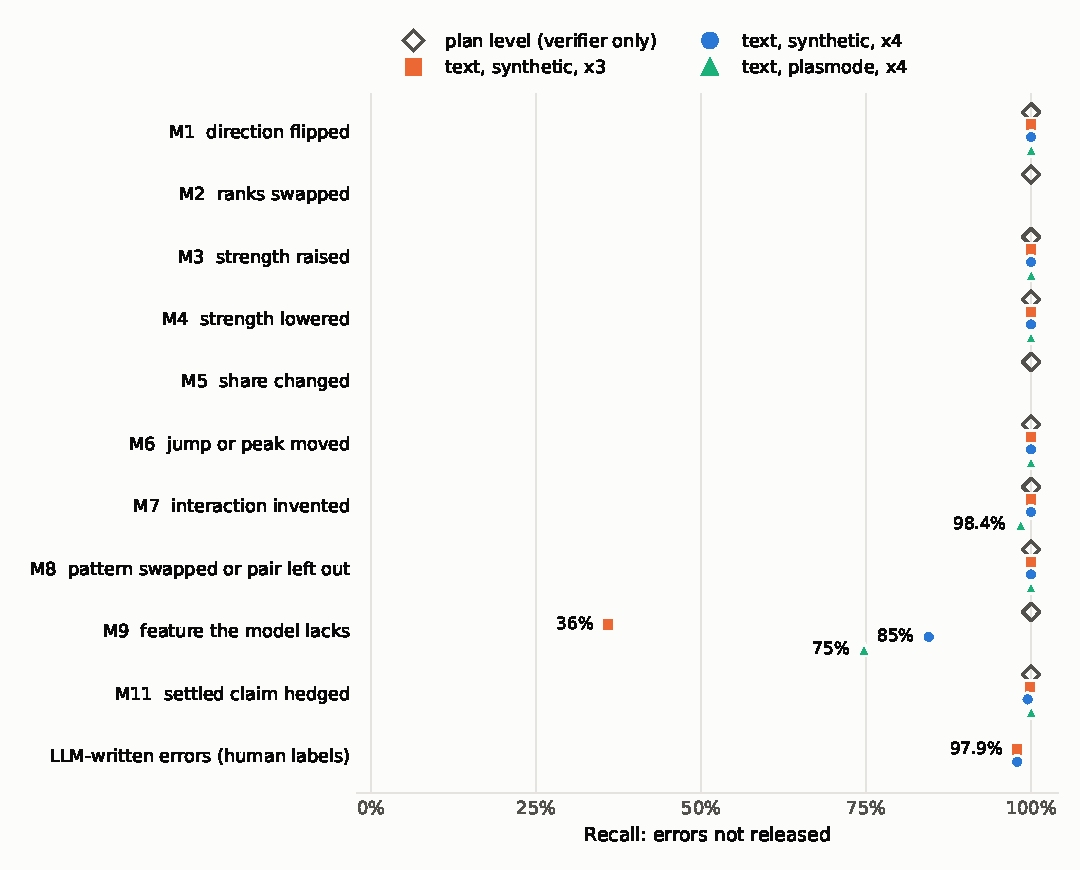
\includegraphics[width=0.72\textwidth]{figures/fig3_recall.pdf}
\caption{Recall per mutation operator. Plan level (gray) is 100\% for every operator on both tiers. At text level
the round trip keeps it except for a feature the model does not have. M2 and M5 (ranks, shares) have no text-level
marks: template texts do not state them. M10 (a strict direction word swapped with ``mostly'') has no row: it has no
label, so it has no recall.}
\label{fig:recall}
\end{figure}

\paragraph{The gate's cost: false alarms.} On LLM-written text the round trip blocks correct sentences when a reading
misreads them. We labeled every claim a fresh round trip blocks in the released texts of E3: 7.7\% of correct texts
(7.9\% if one boundary case counts as a false alarm) are blocked with the earlier extractor and 14.3\% with the final
one, which reads more claims and catches more
invented features. The misreadings are systematic (a ``steepest rise'' read as a jump, a hedge moved onto a settled
statement, a hedge word read as ``mostly'') and can be fixed with deterministic checks of the reading. A false alarm
costs a repair round or the template text, not a wrong statement.

\paragraph{E3: the gate as a control.} Each writer draft is scored with the gate off (the first draft) and on (the
released text) by three readings apart from the gate's own. With Claude Haiku~5.5 as writer (\dsl{claude-haiku-5-5},
run on 15 October 2026; 640 runs outside the two pilot datasets), the share $P_U$ of texts stating a claim false of
$M$ falls from 58.5\% to 4.5\% as read, a control effectiveness $E_U = 1 - P_U(\text{on}) / P_U(\text{off})$
\citep{garcialorite2026distributional} of 0.92 (Table~\ref{tab:e3}). The readings themselves misread: with
author-reviewed labels on every released text with a false claim and on a random sample of 40 first drafts, $P_U$
falls from 20.5\% (95\% interval 13.0--29.5\%) to 0.16\%, and $E_U$ is 0.99, at least 0.94 in the worst case. The one
confirmed error still released is an over-cautious hedge. What first drafts get wrong is mostly shape and uncertainty:
stated jumps the model does not have and hedges on settled facts. The handover is the strongest lever on the first
draft: with the certified statements (H2), 35\% of Haiku's first drafts state a claim false of $M$ against 82\% with
the facts alone (H1), repairs take 1.08 rounds instead of 1.46, and 14\% of runs end in the template instead of 64\%.
With Claude Sonnet~5.5 (\dsl{claude-sonnet-5-5}, 15 October, 64 runs), $P_U$ falls from 25\% to 0\%. A self-hosted
open-weight writer (\dsl{qwen3.8:27b}, 27.8B parameters in 4-bit NVFP4 weights, run with Ollama on a laptop with
24~GB of memory on 17 October; writer cost \$0, 64 runs) behaves like Sonnet~5.5 rather than a weak writer: $P_U$
falls from 28.1\% to 1.6\% ($E_U = 0.94$), 89\% of texts are released and 5\% end in the template (Sonnet: 25.0\%, 88\%
and 5\%; Haiku: 58.5\%, 49\% and 39\%), so the gate's guarantee carries to a writer a bank can host on its own
hardware. The gain is largest where drafts are weakest: pairs and near-flat features (Figure~\ref{fig:faith}). Against $T$, the
gate cuts the share of claims that are false from 11.6\% to 7.6\% (hedges excluded, since $T$ has no bands); what
remains is the models' error from E1, which no check of the text can see. A Haiku run costs \$0.002.

\begin{table}[t]
\centering\footnotesize
\caption{Survival, control effectiveness and cost, outside the pilot datasets. $P_U$: texts with a claim false of
$M$, as read by three scoring readings; the second row replaces the readings' verdicts with author-reviewed labels;
the third and fourth split the first by handover.}
\label{tab:e3}
\setlength{\tabcolsep}{3pt}
\begin{tabular}{p{3.7cm}p{1.7cm}p{2.1cm}p{1.1cm}p{1.9cm}p{1.1cm}p{1.6cm}p{1.1cm}}
\toprule
\textbf{Writer, setting} & \textbf{runs} & \textbf{released / reduced / template / escalate} & \textbf{repair rounds (mean)} & \textbf{$P_U$ before} & \textbf{$P_U$ after} & \textbf{$E_U$} & \textbf{cost per run} \\
\midrule
Claude Haiku 5.5, global (E3) & 640 & 49\% / 12\% / 39\% / 0\% & 1.27 & 58.5\% & 4.5\% & 0.92 & \$0.0023 \\
Claude Haiku 5.5, global, with human labels & 40 drafts, all released texts with a false claim &  &  & 20.5\% (95\% interval 13.0\%–29.5\%) & 0.16\% & 0.99 (worst case 0.94) &  \\
Claude Sonnet 5.5, global (E3 subset) & 64 & 88\% / 8\% / 5\% / 0\% & 0.78 & 25.0\% & 0.0\% & 1.00 & \$0.0184 \\
Qwen3 27B, self-hosted, global (E3 subset) & 64 & 89\% / 6\% / 5\% / 0\% & 0.86 & 28.1\% & 1.6\% & 0.94 & \$0.0006 \\
Claude Haiku 5.5, adverse-action notices (local spot check) & 52 & 62\% / 27\% / 12\% / 0\% & 1.31 & 47.1\% & 3.8\% & 0.92 & \$0.0011 \\
\bottomrule
\end{tabular}

\end{table}

\begin{figure}[t]
\centering
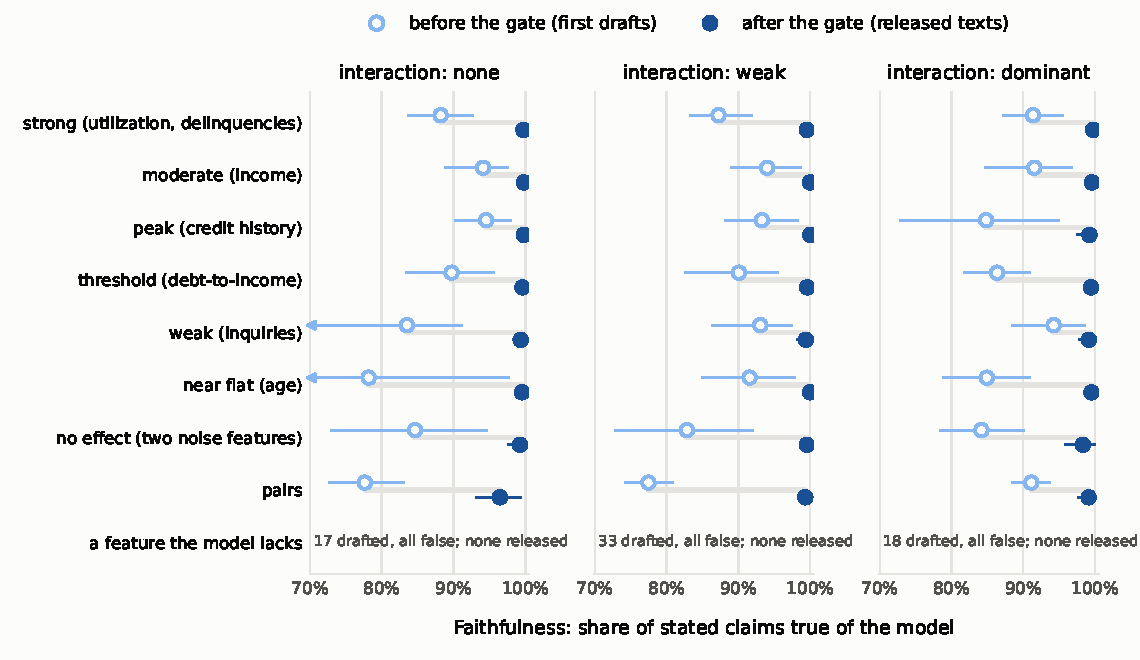
\includegraphics[width=\textwidth]{figures/fig4_faithfulness.pdf}
\caption{Faithfulness (share of stated claims true of $M$) before and after the gate, by feature role and interaction
level; Claude Haiku~5.5 as writer, outside the pilot datasets; 95\% intervals from a bootstrap over datasets. After
the gate the values are a lower bound, since the scoring readings' misreadings count as false.}
\label{fig:faith}
\end{figure}

\paragraph{A local spot check: adverse-action reasons.} Additive models give each term's exact contribution to the gap
between a declined applicant's score and the average score of the 500 approved applicants closest to the cutoff, a
simplified, unweighted version of the comparable passing applicants of \citet{sudjianto2026evidence}; the planted terms
give the true reasons. Three local claim types (a reason's rank, a principal reason above 10\% of the gap and among the
first four, and ``higher'' or ``lower'' than the comparable approved) use the same three-valued rule, with bands from
the same refits. On 52 notices (seed 2, $n=50{,}000$, both models; 54 minus the two of the pilot), the writer's first
drafts state a claim false of $M$ in 47\% of notices (24 of the 51 that could be scored), the released ones in 4\% (2
of 52), and both remaining cases are misreadings by the scoring readings. Of the 76 reasons stated in the 46 released
notices that the true process would also decline, 74 are principal reasons under $T$. Two findings matter for
practice. In 12 notices no principal
reason can be certified, all of them narrow declines whose score gap's band crosses zero; the gate releases them with
hedged reasons, and whether such a notice is acceptable is a question for the regulation, not the gate. And in 6
notices the model declines an applicant whom $T$ rates no riskier than the comparable approved: a faithful notice for
a decision the true process would not make.

\section{Worked example}

One XGB2 model on the synthetic tier (dominant interactions, $n = 50{,}000$; one of the two pilot datasets, on which
the prompts were shaped), handover without certified statements, first draft of Claude Haiku~5.5. The writer reads, among other facts, ``\dsl{dti}: share of importance 5.5\% (95\%
band 4.7\% to 6.3\%)'' and writes ``Debt-to-income ratio has at most a weak effect'', with the claim
\dsl{strength("dti") == "weak"}. The band crosses the 5\% edge between weak and moderate, so the claim is
undecidable; the other twelve claims are certified. The repair message names the band and the two classes it spans,
and the writer answers ``Debt-to-income ratio has a weak to moderate effect'', which is certified. The round trip then
reads the text three times; what it finds beyond the plan is certified, a statement without a DSL form and without a
number (``risk rises steadily'') is flagged, and the text is released after one repair round, at seven calls and
\$0.0025.

The same data show why the gate checks against the model. The planted sign flip (recent inquiries raise the risk for
short credit histories and lower it for long ones) is certified for the EBM (effects $+1.11$ and $-0.56$, both
significant) but undecidable for XGB2 (effects $+0.94$ and $-0.09$, the second not significant). The gate lets the EBM
text say ``the effect reverses'' and holds the same sentence back for XGB2. Both texts are faithful to their model;
$T$ sides with the EBM. The appendix gives the full trace and the EBM's version, whose first draft states a jump the
model does not have.

\section{Limits and next steps}

The outcomes are planted in both tiers; the lexicon's thresholds are fixed by us and not yet validated with human
readers; the writers span two Claude models and one open-weight model, still a narrow sample; and the extractor that
reads texts back is itself an LLM, whose misreadings are the gate's main cost and inflate unlabeled error rates. Most
labels were proposed by the AI assistant that built the pipeline and reviewed by the author (see the statement on AI
use), so they are not independent of it. Three limits of the frozen
design are reported as found: the location rule on count features, a readable handover that draws a gradual rise as
a few large steps (which invites jump claims), and a 95\% band rule that sometimes withholds a claim that 96 of 100
refits support. Next steps are real credit data with a human agreement study of the lexicon, deep gradient boosting
with exact local allocations \citep{nair2022adverse}, and the full local case with weighted references
\citep{sudjianto2026evidence}.

\section{Conclusion}

For a model-risk team, the gate is a control on the text, not on the model. It certifies that every released
statement is true of the fitted model at the resolution of its bootstrap bands, and it holds back or hedges what the
data leave open; it cannot certify that the model is right about the world, which stays with model validation. On
these data, one in five of a small writer's first drafts states something false about the model, and after the gate
one of 640 released texts does (author-reviewed labels), at about \$0.002 per explanation; the gate's own misses and
false alarms are measured, not assumed. It belongs where a bank already checks documentation: after the model is
validated, and before a generated explanation, report or adverse-action notice is used.

\section*{Reproducibility and use of AI tools}

\paragraph{Reproducibility.} The code, the frozen prompts and lexicon, every LLM answer as received, the run traces
and the labels are in the repository (see the title page). The fitted models' facts and bootstrap draws (457~MB) are
not: they come as an archive attached to the repository, together with the TaiwanCredit file. With it,
\dsl{python -m verifier\_gate.experiments.reproduce} re-derives every number, table and figure offline in about seven
minutes and checks each output against the committed one. Without it, the same command refits every model from the
fixed seeds, which takes about six hours and downloads the TaiwanCredit data \citep{yeh2009uci}.

\paragraph{Use of AI tools.} The code, the analyses and a first draft of this text were written with an AI coding
assistant (Claude Code, Anthropic) under the author's direction. The author made the design decisions, reviewed every
number and claim in the text against its source, and is responsible for them. The assistant also helped to label. The
100 LLM-written mutants of E2 were labeled by the author without the gate's verdicts and then reviewed against the
lexicon, with the assistant reading each sentence into claims; the two passes agree on 78 of 86 decisive labels. The
false-alarm labels and the E3 labels were proposed by the assistant, each with a reason, and reviewed by the author,
who changed one. These are the paper's author-reviewed labels. The LLMs under study, the writers and the extractor, are
separate from the assistant.

\bibliographystyle{plainnat}
\bibliography{references}

\clearpage
\appendix
\section{Tables}

\begin{table}[H]
\centering\footnotesize
\caption{Local claims, about one declined applicant.}
\label{tab:dsl-local}
\begin{tabular}{p{3.3cm}p{4.5cm}p{7cm}}
\toprule
\textbf{Words in the text} & \textbf{DSL claim} & \textbf{Meaning (judged on the whole 95\% band)} \\
\midrule
“a principal reason”, “a key reason for the decision” & \texttt{principal\_reason("x")} & x pushes the score towards the decline by at least 10\% of the gap to comparable approved applicants, and is among the four largest such factors \\
“the main reason”, “the first reason” & \texttt{reason\_rank("x") == 1} & x pushes the score towards the decline more than any other factor \\
“the second reason”, “the third reason” & \texttt{reason\_rank("x") == 2} (or 3, 4) & x is the second (third, fourth) largest factor pushing towards the decline \\
“one of the two main reasons”, “the second or third reason” & \texttt{reason\_rank("x") in (1, 2)}, \texttt{reason\_rank("x") in (2, 3)} & one of consecutive ranks \\
“high x”, “x is higher than for approved applicants” & \texttt{higher\_than\_reference("x")} & the applicant's value is above the median of comparable approved applicants \\
“low x”, “a short x”, “few x” & \texttt{lower\_than\_reference("x")} & the applicant's value is below that median \\
“the data do not settle whether ...” & \texttt{unsettled(<any claim above>)} & the facts leave that claim open \\
\bottomrule
\end{tabular}

\end{table}

\begin{table}[H]
\centering\footnotesize
\caption{The lexicon's thresholds (lexicon v2, frozen).}
\begin{tabular}{p{4.2cm}p{10.8cm}}
\toprule
\textbf{Threshold} & \textbf{Value} \\
\midrule
strength classes (share of importance) & negligible < 2\% ≤ weak < 5\% ≤ moderate < 15\% ≤ strong \\
detectable effect & simultaneous band excludes 0 on more than 5\% of the data, or a significant net change \\
“about x\%” & within 2\% points or 10\% of the share \\
“mostly” (exception mass) & a detected reversal on at most 10\% of the data \\
jump / peak location (window w) & 2\% of the 5th-95th percentile range; on counts, the gap between observed values (v2) \\
jump size & at least 50\% of the term's range, significant \\
interaction present & pair share band at or above 2\% and a significant interaction contrast \\
band level & 95\%, from 100 Poisson bootstrap refits; curves: simultaneous (sup-t) bands \\
\bottomrule
\end{tabular}

\end{table}

\begin{table}[H]
\centering\footnotesize
\caption{The benchmark. Synthetic tier (top), plasmode tier (middle), planted pairs (bottom).}
\label{tab:benchmark}
\begin{tabular}{llp{3.4cm}p{4.6cm}r}
\toprule
\textbf{Feature} & \textbf{Role} & \textbf{Distribution} & \textbf{Planted shape} & \textbf{Share (no interaction)} \\
\midrule
utilization & strong & Beta(2, 3) & increasing, steeper above 0.6 & 40\% \\
n\_delinquencies & strong & min(Poisson(0.8), 6) & increasing, saturating & 24\% \\
income & moderate & lognormal, median 50,000, σ 0.5 & decreasing (−log income) & 13\% \\
history\_months & peak & uniform 6 to 360 & decreasing, with a bump at 36 months (rising on 7\% of the data) & 10\% \\
dti & threshold & uniform 0 to 0.6 & a step up at 0.43 & 8\% \\
n\_inquiries & weak & Poisson(1.5) & increasing (linear) & 4\% \\
age & near flat & uniform 21 to 75 & decreasing (linear) & 1\% \\
noise\_1 & noise & N(0, 1) & zero & 0\% \\
noise\_2 & noise & N(0, 1) & zero & 0\% \\
\bottomrule
\end{tabular}
\\[6pt]
\begin{tabular}{llp{7cm}r}
\toprule
\textbf{Feature} & \textbf{Role} & \textbf{Planted shape} & \textbf{Share (no interaction)} \\
\midrule
PAY\_0 & strong & the real-label EBM's, per status value & 40\% \\
LIMIT\_BAL & strong & decreasing, smooth & 24\% \\
BILL\_AMT1 & moderate & increasing, smooth & 13\% \\
PAY\_AMT1 & moderate & decreasing, smooth & 10\% \\
PAY\_AMT2 & threshold & a step down at 2,000 & 8\% \\
AGE & weak & increasing, smooth & 4\% \\
EDUCATION & near flat & linear in the code, clipped to 1 to 3 & 1\% \\
BILL\_AMT2 & correlated null & zero; Spearman 0.91 with BILL\_AMT1 & 0\% \\
PAY\_AMT3 & noise & zero & 0\% \\
\bottomrule
\end{tabular}
\\[6pt]
\begin{tabular}{lllrrr}
\toprule
\textbf{Tier} & \textbf{Pair} & \textbf{Pattern} & \textbf{Share, none} & \textbf{Share, weak} & \textbf{Share, dominant} \\
\midrule
synthetic & utilization \& n\_delinquencies & amplification & 0\% & 3\% & 21\% \\
synthetic & history\_months \& n\_inquiries & sign flip & 0\% & 6\% & 6\% \\
plasmode & PAY\_0 \& EDUCATION & amplification & 0\% & 3\% & 21\% \\
plasmode & AGE \& BILL\_AMT1 & sign flip & 0\% & 6\% & 6\% \\
\bottomrule
\end{tabular}

\end{table}

\section{The worked example in full}

The repository holds the full trace, generated from the run: the handover excerpt, the first draft, the plan check,
the repair message, the released text with each claim's verdict and lexicon entry, the round trip, and the EBM
version (file \dsl{worked\_example.md} in the folder \dsl{paper}). Figure~\ref{fig:shapes} shows the planted and
fitted terms of three of its features.

\begin{figure}[H]
\centering
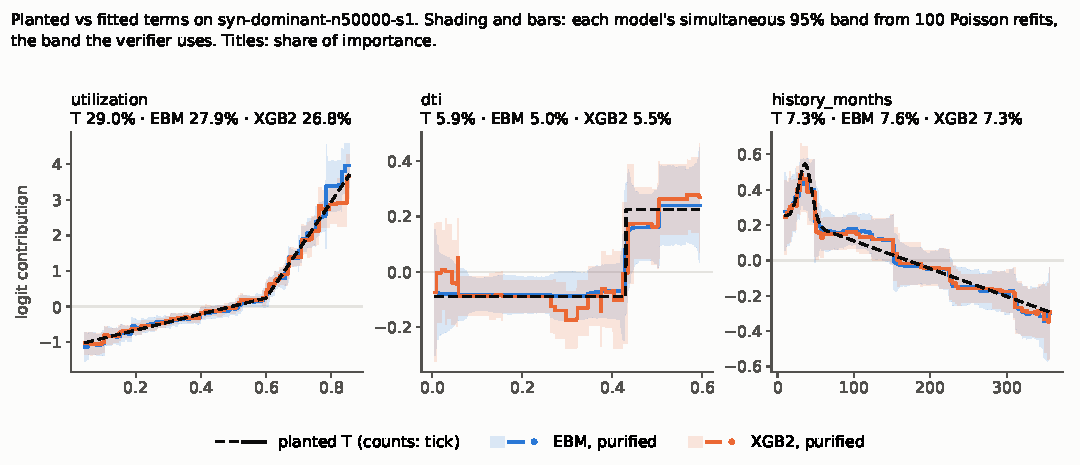
\includegraphics[width=\textwidth]{figures/worked_example_shapes.pdf}
\caption{Planted ($T$) and fitted terms with their simultaneous 95\% bands for utilization, the debt-to-income ratio
and the length of credit history, on the dataset of the worked example.}
\label{fig:shapes}
\end{figure}

\end{document}
